\pagestyle{fancy}
\renewcommand{\theUnit}{3}
\ifthenelse{\isundefined{\UnitPageNumbers}}{}{\setcounter{page}{1}}
\rhead{Chapter \theUnit: Hypothesis Tests}
\lhead{Math 3382: Statistical Theory}
%\lhead{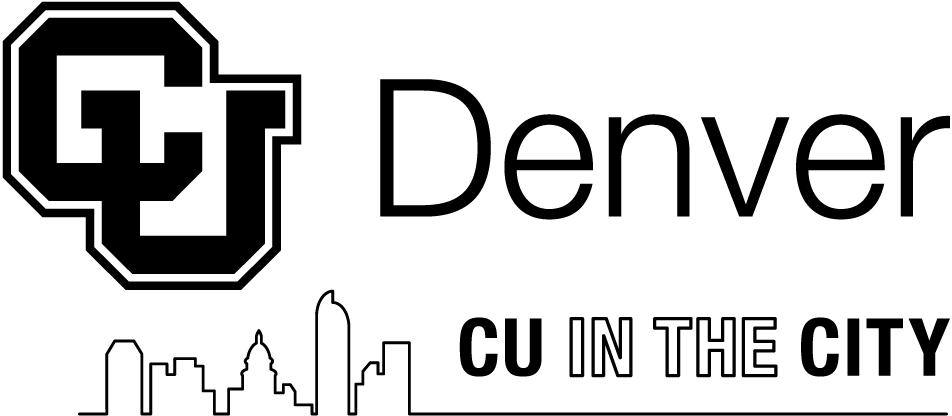
\includegraphics[width=1.25cm]{CUDenver-Logo.png}}
\rfoot{\mypage}
\cfoot{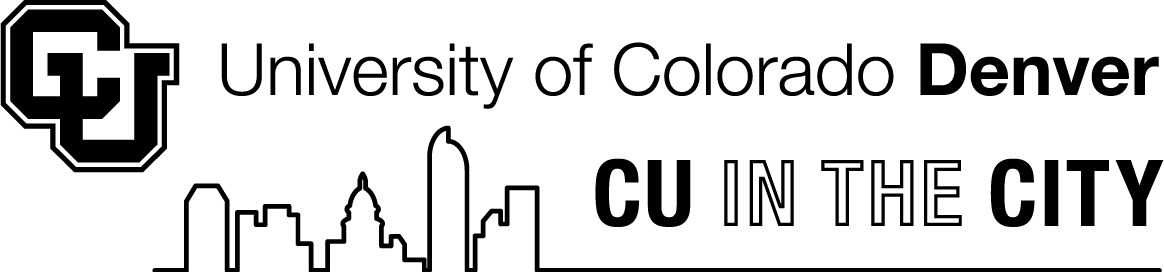
\includegraphics[width=2.25cm]{CUDenver-Logo-coverpage.png}}
\lfoot{Adam Spiegler}
\fancypagestyle{firstfooter}{\footskip = 50pt}
\renewcommand{\footrulewidth}{.4pt}
%%%%%%%%%%%%%%%%%%%%%%%%%%%
\vspace*{-20pt} \thispagestyle{firstfooter}


%\begin{tasks}[counter-format = {(tsk[a])},label-offset = {0.8em},label-format = {\color{black}\bfseries}](2)

\pagebegin{Section 3.3: Permutation Tests}

In the experiment involving evenly-paying versus pay what you order experiment, how can we calculate the $P$-value if we do not know the underlying probability distribution for $T = \mu_{\rm{even}} - \mu_{\rm{control}}$?

\bb[resume]
\ii If how people split the bill does not matter (assuming $H_0$), then the eight values were just randomly split into
two groups of four people, and the actually method of paying has no effect. It could just have turned out that:

\begin{center}
\begin{tabular}{|cccc|}
\hline
\multicolumn{4}{c}{Even-Split}\\
\hline
$\mathbf{\$7.43}$ & $\$8.00$ & $\$8.75$ & $\$13.17$\\
\hline
\end{tabular}
\ \ \ \ \ \ \ \ \ \ \ \ \ \ \ \ \ \ \ \ \ \ \ \ \
\begin{tabular}{|cccc|}
\hline
\multicolumn{4}{c}{Control}\\
\hline
$\$8.50$ & $\$7.90$ & $\$10.85$ & $\mathbf{\$15.00}$\\
\hline
\end{tabular}
\end{center}

\bb
\ii What would be the test statistic for the two samples above? \vspace{1in}
\ii How many different ways can we divide the eight participants into two groups of four? \vspace{1in}
\ee
\ee

\bbox
To perform a \textbf{\colorb{two-sample permutation test}} on data collected from two samples size $m$ and $n$:
\bi
\ii Pool the $m+n$ values together.
\ii Draw a \textbf{\colorb{permutation resample (or resample for short)}  of size $m$ without replacement.}
\ii Use the remaining $n$ observations for the other sample.
\ii Calculate the difference in means or another statistic that compares samples.
\ii Repeat the resamplng process many, many times.
\ii The $P$-value is the proportion of times the random statistics are as or more extreme than the observed difference.
\ei
\ebox

\clearpage

\begin{center}
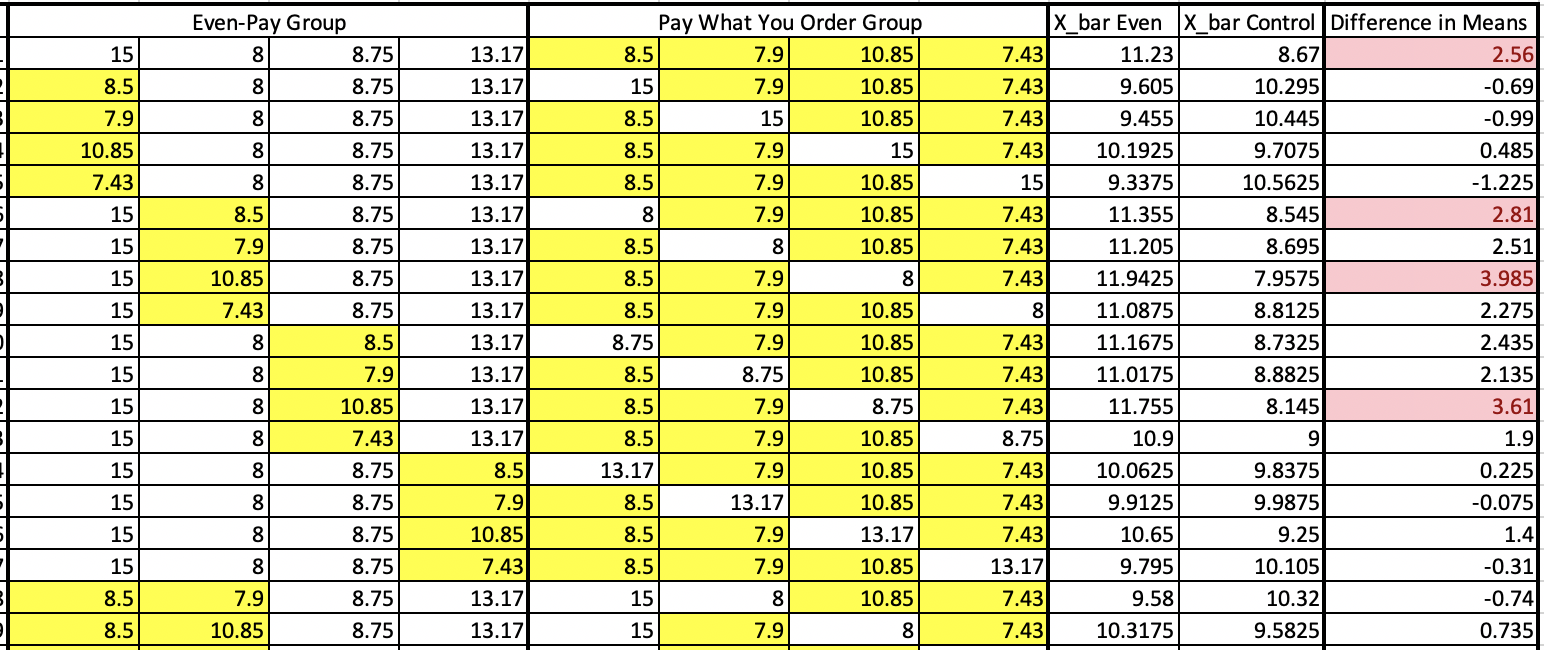
\includegraphics[width=0.95\tw]{19/fig-meal-permutation.png}
\end{center}

Out of the 70 possible ways of splitting the 8 volunteers into two groups (of four people), 7 had a test statistic that is as or more extreme than the observed test statistic, so
\[ P-\mbox{value} = \frac{7}{70} = 0.10.\]


\bb[resume]
\ii The dataset \textit{Beerwings} contains observations from a sample of 30 people at a bar in which three variables were collect: Gender, Beer and Hot Wings. Imagine a researcher wants to perform a hypothesis test to determine whether males eat more hot wings than women. Out of the 15 males, the mean number of wings consumed was $14.53$ with a standard deviation of $3.56$. Out of the 15 females, the mean number of winds consumed was $9.33$ with a standard deviation of $4.50$.

\begin{center}
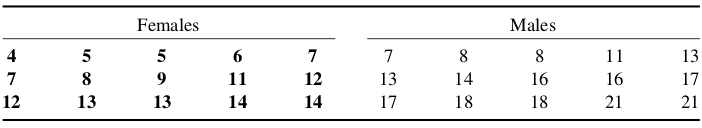
\includegraphics[width=0.75\tw]{19/fig-wings-table.png}
\end{center}

\bb
\ii Write out the null and alternative hypotheses using appropriate notation. \vfill
\ii What can we use as the test statistic? What is the value of the observed test statistic? \vfill
\ii If we want to repeat the previous process, we assume gender has no effect, and group all 30 people together. Then we compare the observed difference in sample means to the difference in sample means in all possible resamples. How many different ways can we split the 30 people into two groups each of size 15? \vfill
\ee
\ee

\clearpage

\bbox
In practice, it takes a lot of time and energy (and money) to generate all possible resamples (without any duplicate resamples). Instead we do the following:
\bi
\ii Create a resample by picking $m=15$ observations without replacement from the pooled data to be one sample (say females)
and let the remaining $n=15$ observations be considered as the males.
\ii Calculate the test statistic, in this case $\bar{x}_{\rm{M}} - \bar{x}_{\rm{F}}$.
\ii Repeat this many, many, many times. The more the merrier!
\ii The $P$-value is the fraction of times the random statistic is as or more extreme than the observed test statistic.
\ei
\ebox

\bb[resume]
\ii Returning the to hot wings example. You will first need to enter the command \textbf{library(resampledata)} to get access to the dataset \textit{Beerwings}.
\bb
\ii Find the observed test statistic:
\begin{lstlisting}
tapply(Beerwings$Hotwings, Beerwings$Gender, mean) 
observed <- 14.533-9.333
\end{lstlisting}
\ii Generate $N=10^5-1$ resamples and calculate the difference in the means for each resample.
\begin{lstlisting}
hotwings <- subset(Beerwings, select = Hotwings, drop = T)
N <- 10^5 - 1
result <- numeric(N)
for (i in 1:N)
{
  index <- sample(30, size = 15, replace = FALSE)
  result[i] <- mean(hotwings[index]) - mean(hotwings[-index])
}
\end{lstlisting}
\ii Calculate the $P$-value, how likely is it to get samples with a difference in means as or more extreme than the observed test
statistic.
\begin{lstlisting}
(sum(result >= observed) + 1)/(N+1)
\end{lstlisting}
\bi
\ii The command $\mbox{result } >= \mbox{ observed}$ creates a vectors of T's and F's depending on whether the resulting difference is greater than or equal to the observed difference.
\ii Then count the number of T's we have and then add 1 to account for the original observed sample.
\ii Finally divide by $N+1$ to to account for the original observed sample.
\ei
\ee
\ee

\clearpage

\pagebegin{Permutation Tests On Other Statistics}

\bb[resume]
\ii (Exercise 3.9) Using the dataset FlightDelays perform the following permutation tests. For each, write out the hypotheses both in
words and with appropriate notation. State what the test statistic is, and find the value of the observed test statistic. Finally, similar to the previous example, construct a permutation distribution for the test statistic, and calculate the $P$-value of the observed test statistic.
\bb
\ii Is the variance of the flight lengths in May different from the variance of the flight lengths in June? Note that the variables FlightLength and Month will be of importance. \textit{Hint: Instead of mean use the variance (var) as the function in tapply.}

\vfill

\ii Is the proportion of times the flights in May were delayed more than 20 minutes different from the proportion of times the flights in June were delayed more than 20 minutes? Note that the variables Delay and Month will be of importance.

\vfill

\ee
\ee

\pagebegin{Section 3.4: Matched Pairs}

\begin{multicols}{2}

In the 2008 Olympics there was a lot of controversy over new swimsuits that possibly provided an unfair advantage to swimmers
which led to new international rules regarding swimsuit materials and coverage. Can a swimsuit really make a swimmer faster?

\medskip

A study\footnote{de Lucas, Balidan, Neiva, Grecco, and Denadai. ``The effects of wetsuits on physiological and biomechanical indices during swimming'', \textit{Journal of Science and Medicine in Sport}} tested whether wearing wetsuits influences swimming velocity. Twelve competitive swimmers swam 1500 meters at maximum speed twice each. Once wearing a wetsuit and once wearing a regular bathing suit. The order of the trials was randomized. Each time, the maximum velocity in meters/sec of the swimmer was recorded.

\columnbreak

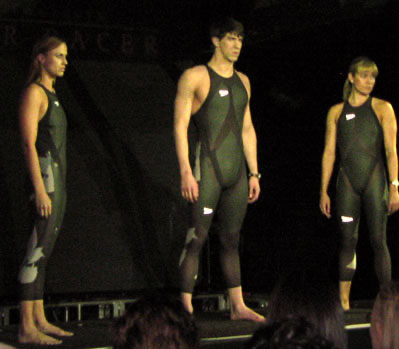
\includegraphics[width=0.35\tw]{19/fig-phelps.jpg}

\end{multicols}

\vspace{0.5in}

\begin{tabular}{|l||c|c|c|c|c|c|c|c|c|c|c|c|}
Swimmer & 1 & 2 & 3 & 4 & 5 & 6 & 7 & 8 & 9 & 10 & 11 & 12 \\
\hline
Wetsuit & $1.57$ & $1.47$ & $1.42$ & $1.35$ & $1.22$ & $1.75$ & $1.64$ & $1.57$ & $1.56$ & $1.53$ & $1.49$ & $1.51$ \\
No Wetsuit & $1.49$ & $1.37$ & $1.35$ & $1.27$ & $1.12$ & $1.64$ & $1.59$ & $1.52$ & $1.50$ & $1.45$ & $1.44$ & $1.41$ \\
\hline
Difference & $0.08$ &  $0.10$ &  $0.07$ &  $0.08$ &  $0.10$ & $0.11$ & $0.05$ & $0.05$ & $0.06$ & $0.08$ & $0.05$ &  $0.10$
\end{tabular}


\bb[resume]
\ii If researchers are testing to see whether the wetsuit makes people swim faster, set up hypotheses for this test. \vfill

\ii What is the observed test statistic? \vfill

\ii Devise of method that we can use permutation resamples to construct a permutation distribution to approximate the null distribution.\ee

\vfill

\clearpage

\bbox
\bi
\ii We do not want to group both samples together and randomly assign to a wetsuit and no wetsuit group since the two samples
are not independent.
\ii We would like to compare each swimmers wetsuit and regular bathing suit velocities.
\ii If there really is no difference, it was random which velocity was the wetsuit and which was the bathing suit.
\ii For each pair, we can randomly assign one velocity as the wetsuit velocity and use the other as the no wetsuit velocity.
\ii Calculate $t= \bar{x}_{\rm{diff}}$, the mean of the paired differences.
\ei
\ebox

\medskip
\begin{tabular}{l||c|c|c|c|c|c|c|c|c|c|c|c}
Swimmer & 1 & 2 & 3 & 4 & 5 & 6 & 7 & 8 & 9 & 10 & 11 & 12 \\
\hline
Wetsuit & $1.57$ & $\mathbf{1.37}$ & $\mathbf{1.35}$ & $1.35$ & $1.22$ & $1.75$ & $1.64$ & $1.57$ & $\mathbf{1.50}$ & $1.53$ & $1.49$ & $1.51$ \\
No Wetsuit & $1.49$ & $\mathbf{1.47}$ & $\mathbf{1.42}$ & $1.27$ & $1.12$ & $1.64$ & $1.59$ & $1.52$ & $\mathbf{1.56}$ & $1.45$ & $1.44$ & $1.41$ \\
\hline
Difference & $0.08$ &  $\mathbf{-0.10}$ &  $\mathbf{-0.07}$ &  $0.08$ &  $0.10$ & $0.11$ & $0.05$ & $0.05$ & $\mathbf{-0.06}$ & $0.08$ & $0.05$ &  $0.10$
\end{tabular}

\smallskip

\colorr{\textbf{The test statistic of the resample above is $\mathbf{t = \bar{x}_{\rm{diff}} = 0.039}$.}} \smallskip


%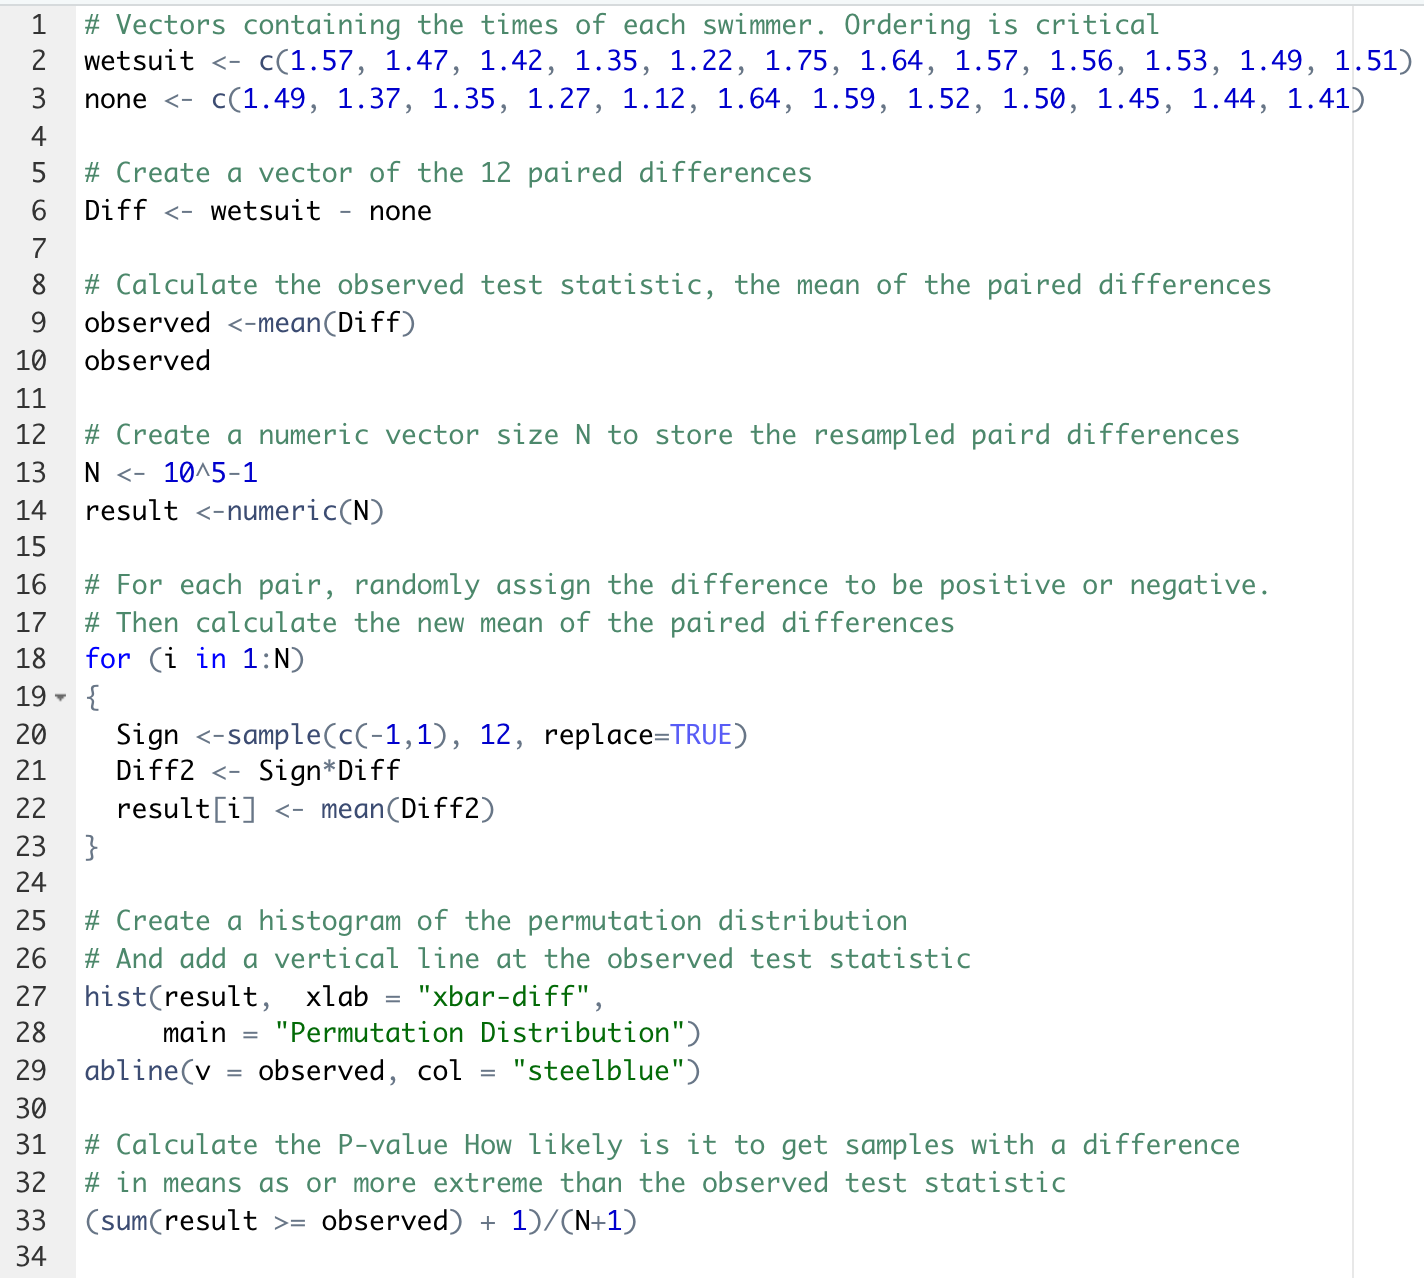
\includegraphics[width=0.85\tw]{10/fig-swimsuit-code.png}

\begin{lstlisting}
# Vectors containing the times of each swimmer. Ordering is critical
wetsuit <- c(1.57, 1.47, 1.42, 1.35, 1.22, 1.75, 1.64, 1.57, 1.56, 1.53, 1.49, 1.51)
none <- c(1.49, 1.37, 1.35, 1.27, 1.12, 1.64, 1.59, 1.52, 1.50, 1.45, 1.44, 1.41)

# Create a vector of the 12 paired differences
Diff <- wetsuit - none

# Calculate the observed test statistic, the mean of the paired differences
observed <-mean(Diff) 
observed

# Create a numeric vector size N to store the resampled paird differences
N <- 10^5-1
result <-numeric(N)

# For each pair, randomly assign the difference to be positive or negative.
# Then calculate the new mean of the paired differences
for (i in 1:N)
{
  Sign <-sample(c(-1,1), 12, replace=TRUE)
  Diff2 <- Sign*Diff
  result[i] <- mean(Diff2)
}

# Create a histogram of the permutation distribution
# And add a vertical line at the observed test statistic
hist(result,  xlab = "xbar-diff",
     main = "Permutation Distribution")
abline(v = observed, col = "steelblue")

# Calculate the P-value How likely is it to get samples with a difference
# in means as or more extreme than the observed test statistic
(sum(result >= observed) + 1)/(N+1)
\end{lstlisting}

\clearpage

\bb[resume]
\ii (Exercise 3.15) Is there a difference in the price of groceries sold by Target and Walmart? The dataset \textit{Groceries} contains a sample of grocery items and their prices advertised on their respective websites on a specific day.

\bb
\ii First load the data into two separate vectors of Walmart and Target prices.
\begin{lstlisting}
library(resampledata)
target <-Groceries$Target
walmart <-Groceries$Walmart
\end{lstlisting}

\ii Calculate the mean price for each retailer. \vspace{1in}
\ii Is there a difference in the price of groceries sold by Target and Walmart? Set a hypothesis, and compute the $P$-value for the observed test statistic by modifying the code of the previous example.
\ee
\ee
